\documentclass[border=8pt]{standalone}
\usepackage{tikz}
\usetikzlibrary{arrows.meta}

\begin{document}

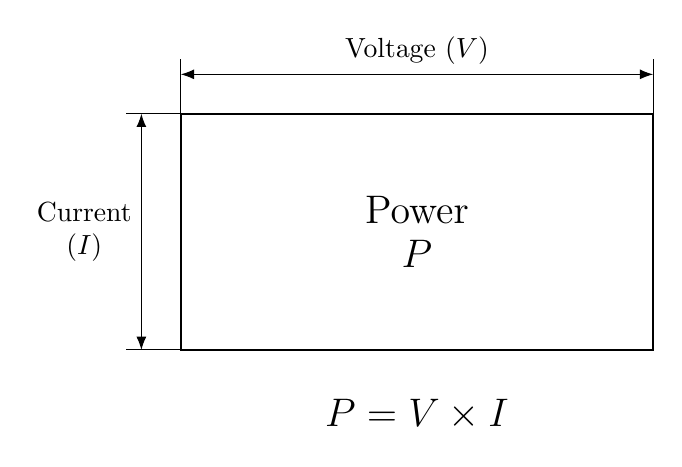
\begin{tikzpicture}[>=Latex]

% Rectangle dimensions are illustrative only.
% They are not intended to represent numerical values.
\def\rectwidth{6}
\def\rectheight{3}

% Power rectangle
\draw[thick]
    (0,0) rectangle (\rectwidth,\rectheight);

% Power label
\node[align=center] at (\rectwidth/2,\rectheight/2)
    {\Large Power\\[4pt]\Large $P$};

% Voltage dimension across the top
\draw[<->]
    (0,\rectheight+0.5)
    -- node[above] {Voltage ($V$)}
    (\rectwidth,\rectheight+0.5);

% Extension lines for voltage
\draw
    (0,\rectheight)
    -- (0,\rectheight+0.7);

\draw
    (\rectwidth,\rectheight)
    -- (\rectwidth,\rectheight+0.7);

% Current dimension along the left side
\draw[<->]
    (-0.5,0)
    -- node[left, align=center] {Current\\($I$)}
    (-0.5,\rectheight);

% Extension lines for current
\draw
    (0,0)
    -- (-0.7,0);

\draw
    (0,\rectheight)
    -- (-0.7,\rectheight);

% Relationship underneath
\node[below] at (\rectwidth/2,-0.5)
    {\Large $P = V \times I$};

\end{tikzpicture}

\end{document}